\documentclass[10pt]{article}
\usepackage[margin=1in]{geometry}
\usepackage{graphicx}
\usepackage{booktabs}
\usepackage{amsmath}
\usepackage{fontspec}
\usepackage[hidelinks]{hyperref}
\usepackage{xurl}
\usepackage{microtype}
\usepackage[font=small]{caption}
\title{Run the Real Tests\\[4pt]\large Scoring every intermediate step of 345 Gemma 4 coding-agent runs: agents rarely lose a fix, often trust a wrong one, and are right twice as often when they check with the repository's own tests}
\author{Sundar Shahi Thakuri\\ Independent researcher\\ \small Gemma 4 Developer Agent Paper Track}
\date{November 2026}
\begin{document}
\maketitle
\begin{center}\fbox{\begin{minipage}{0.95\linewidth}\small\textbf{Key findings}\begin{itemize}\setlength\itemsep{2pt}\item When a Gemma 4 31B agent's check passed, the hidden tests also passed \textbf{68\% of the time if it ran the repository's test suite, and only 38\% if it ran a script it wrote itself}. Within the same run, the repository suite was never the less reliable signal (22 runs to 0).\item Ending a run at the agent's first passing test \textbf{loses 13 fixes and gains none} (p = 0.0002).\item Agents almost never throw away a working fix: 0 of 72 E4B runs and 2 of 273 31B runs did. When 31B broke a working version, it usually put it back by itself.\item Most failures never reach a working fix at all. Half of the failed 31B runs edited exactly the right lines and still got it wrong.\item We release 1,431 intermediate agent states, each labelled pass or fail by the official hidden tests, plus the tools that produced them.\end{itemize}\end{minipage}}\end{center}
\section*{Abstract}
A coding agent edits a repository many times before it submits a patch, but only the submitted patch is scored. We score all of the steps in between. We record the workspace after every file-changing action and run the competition's official hidden tests on each version. The data cover Gemma 4 E4B running the official sample agent on 72 valid tasks, and 273 Gemma 4 31B runs from 17 agent configurations, rebuilt from public logs. In total that is 1,431 distinct intermediate states, all scored. Three results follow. First, agents seldom lose a fix they already had (2 of 345 runs), so checkpoint-and-undo machinery has little to recover. Second, the agent's own sense that its fix works is unreliable: only 48\% of 31B's passing test runs coincided with a correct workspace, and 29\% for E4B. Third, the kind of check matters. A pass from the repository's own test suite was right 68\% of the time, while a pass from a scratch reproduction script was right 38\% of the time (Fisher p = 2$\times 10^{-8}$). For people building small agents, the cheapest improvement is to make the agent confirm its fix with the project's real tests, and not to trust an early green result.

\section*{Introduction}
Small local models struggle with multi-step software engineering, and most work on this competition tries to help the agent find the right code or write a better fix. We looked at something in between: what happens to a fix after the agent writes it.

There are two reasons to look. The first is that a good fix can be lost. Kim et al. [1] found frontier agents that wrote the reference fix word for word in the middle of a run and then overwrote it. If small models did this often, a harness could keep checkpoints and return the best one, with no extra model calls. The second is that the agent decides when it is done. It writes a reproduction script, runs it, sees it pass and submits. If that signal is wrong, the agent stops too early or submits a broken patch.

To measure both, we need to know whether each intermediate version is correct, not just the final one. So we ran the hidden tests on every version an agent produced.

We answer three questions:

\begin{enumerate}\setlength\itemsep{2pt}\item \textbf{How often does an agent have a working fix and then submit a broken one?}\item \textbf{When the agent believes its fix works, how often is it right, and does it matter what it tested with?}\item \textbf{Could a simple rule, using only what the agent knew at the time, pick a better version than the one it submitted?}\end{enumerate}
\section*{Related work}
Kim et al. [1] split 16,758 frontier-model trajectories into search, read and edit stages and compared them with the reference patch. They report that 60--69\% of failures reach and edit the right code, and they name the reach-then-overwrite pattern \emph{coherence collapse}. We run the hidden tests on each state instead of comparing it with the reference, so any correct patch counts, and we study small open models. Gupta et al. [4] analyse backtracking in 154k trajectories, and Cuadron et al. [5] show that more reasoning can hurt agent performance.

Other methods pick among patches. SWE-Search [6] searches over repository states with backtracking. Agentless [7] and CodeMonkeys [8] generate many candidate patches and use tests to choose one. They choose between separate attempts; we ask whether a choice inside one attempt helps.

Within this competition, Papasani [2] audited the public tasks and found that 14.7\% of deliberately broken fixes still pass the tests. Vein05 [9] found that showing 31B the existing tests its patch breaks made it damage correct patches, a first sign that agent-side test signals mislead. A pre-registered study [10] looks at lost edits when the context is compacted, and sigongjoa [11] show that a 2B agent often cannot apply its edits at all.

\section*{Method}
\subsection*{Which tasks count}
The public development set has 129 tasks. We ran the official verifier on each one twice, once with the reference fix (it should pass) and once with no change (it should fail). 72 tasks behave correctly: 43 from rich and 29 from fastapi. These include all 68 tasks from Papasani's independent audit [2]. Every result below uses only these 72.

\subsection*{Agents}
\textbf{Gemma 4 E4B, run live.} We ran the official sample submission with only the model name changed. It has the six workspace tools, the three graph tools, a code-analyzer sub-agent, temperature 0.2 and a 4,096-token thinking budget. The sample's own budget of 10 tool calls and one minute per task is too short to study, so we allowed 100 tool calls, 100 turns and 10 minutes. It ran with vLLM on four L4 GPUs.

\textbf{Gemma 4 31B, rebuilt from logs.} Our own 31B run was stopped when the weekly GPU quota ran out. Instead we used 298 public 31B runs from Papasani [2], covering 17 agent configurations on 67 of the valid tasks.

\subsection*{Recording every version}
For the live run, we wrapped the harness's file-editing, shell and submit functions. After each call, the wrapper saves the workspace diff the same way the harness computes a submission, using a private copy of git's index so the agent sees nothing different. The agent's prompts, tools and budgets are unchanged.

For the logged runs, we unpacked each task's repository and re-applied every edit in order with the harness's own edit-matching function, re-running any shell command that might change files. We kept a run only if every re-run command behaved as logged and the final rebuilt diff equals the patch the original run submitted. 273 of 298 runs passed both checks.

\subsection*{Scoring}
Each distinct version was scored by the official verifier in a fresh sandbox: apply the diff, add the hidden tests, run pytest. That is 1,312 versions for 31B and 119 for E4B, with none skipped. Versions scored twice always got the same verdict. As a check on the whole pipeline, our verdict on each run's final version matched the originally logged result in every case (269 of 269 for 31B, 66 of 66 for E4B).

We call a run's version \textbf{working} if it passes the hidden tests. A \textbf{check} is any command the agent runs to test its work: a test runner such as pytest, or a Python script named like repro, verify, test, check or debug. We split checks into those that run the \textbf{repository's test suite} (the \texttt{tests/} directory, or pytest with no file named) and those that run the agent's \textbf{own scratch script}.

\section*{Results}
\subsection*{The agent's own checks are often wrong}
\begin{figure}[h]\centering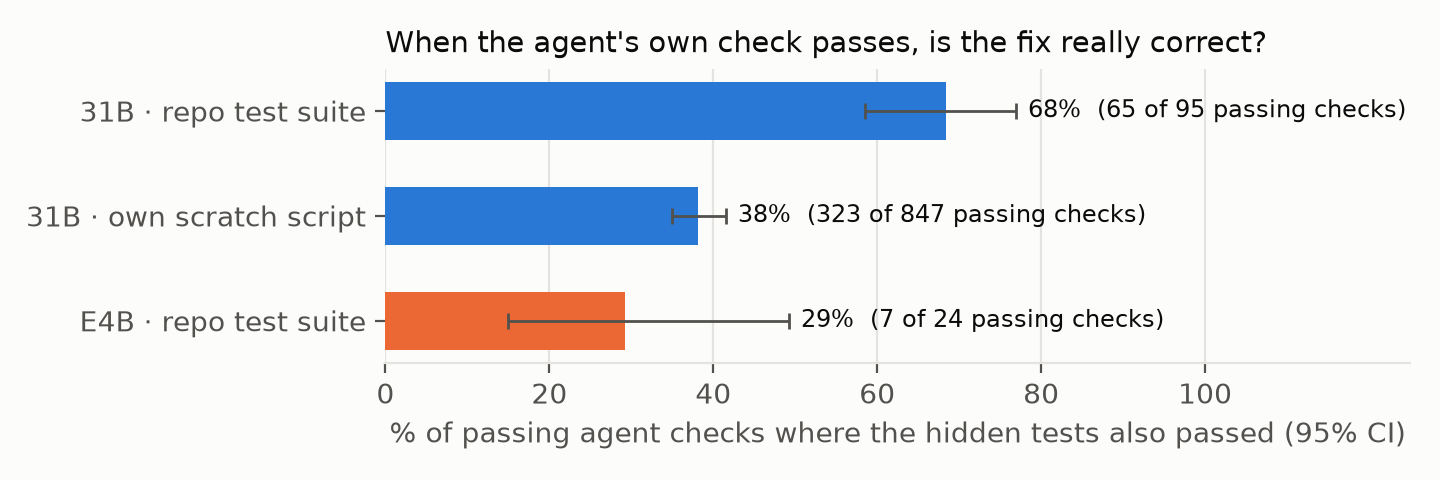
\includegraphics[width=\linewidth]{fig/fig3_checks.png}\caption{How often a passing agent check is right.}\end{figure}
When 31B ran a check and it passed, the workspace was actually working only part of the time. The difference between kinds of check is large:

\begin{center}\small\begin{tabular}{lr}\toprule
\textbf{Check that passed} & \textbf{Workspace really working} \\ \midrule
31B, repository test suite & 65 of 95 (68\%) \\
31B, own scratch script & 323 of 847 (38\%) \\
E4B, repository test suite & 7 of 24 (29\%) \\
\bottomrule\end{tabular}\end{center}
The gap is significant (Fisher exact test, p = 2$\times 10^{-8}$). Checks from one run are related, so we also compared the two kinds inside the same run. In the 40 runs where 31B used both, the repository suite was the more reliable signal in 22 runs, the scratch script in none, and 18 were ties.

The likely reason is simple. A scratch script tests the agent's own reading of the issue, so it can pass while the real requirement is still unmet. The repository's tests encode what the maintainers expect. They are not perfect either: an existing suite that passes mainly shows nothing broke, which may be why E4B's suite passes were right less often. One caution: agents may run the full suite later in a run, when the fix is already better, so part of the gap could be timing.

\subsection*{Trusting the first green result costs fixes}
We tested four rules for picking which version to submit, using only information the agent had at that moment. Every version these rules pick was actually reached and scored, so this needs no new model runs.

\begin{center}\small\begin{tabular}{lrr}\toprule
\textbf{Rule (31B, 273 runs)} & \textbf{Runs solved} & \textbf{Change vs submitted} \\ \midrule
Submit what the agent submitted & 163 & --- \\
Submit the final workspace & 163 & 0 \\
Submit the version at the last passing check & 162 & --1 \\
Submit the version at the first passing check & 150 & --13 (p = 0.0002) \\
\bottomrule\end{tabular}\end{center}
No rule did better than the agent's own submission. Stopping at the first passing check made things significantly worse, because that check is so often wrong. For E4B every rule gave the same 9 solved runs.

\subsection*{Agents rarely lose a fix, and 31B fixes its own breaks}
\begin{center}\small\begin{tabular}{lrrrr}\toprule
\textbf{} & \textbf{Runs} & \textbf{Solved} & \textbf{Working at some point} & \textbf{Lost a working fix} \\ \midrule
E4B & 72 & 9 & 9 & 0 \\
31B & 273 & 163 & 165 & 2 (0.7\%) \\
\bottomrule\end{tabular}\end{center}
E4B usually makes one change and submits it: the median run has a single version. A model that rarely revises cannot lose much by revising. 31B revises more, with a median of four versions, but lost a working fix in only 2 runs. The 95\% interval runs from 0.2\% to 2.6\%, so even in the worst case, recovering every lost fix would add under three points.

31B did break working versions 13 times in 12 runs. It repaired 11 of those breaks before the end, and 9 of the repairs were exact reverts to the earlier working version, usually within two tool calls. Six repairs came right after one of its checks failed. The model already runs a small undo loop of its own: edit, check, put it back.

\begin{figure}[h]\centering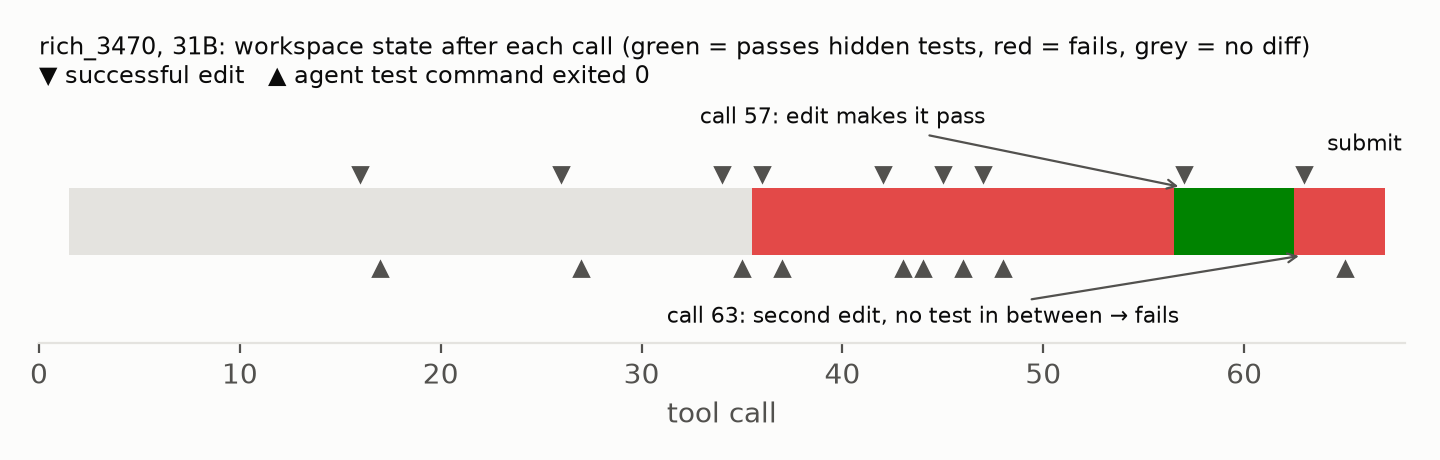
\includegraphics[width=\linewidth]{fig/fig2_lost_fix.png}\caption{One of the two lost fixes, step by step.}\end{figure}
Figure 2 shows one of the two lost fixes. At step 57 an edit makes the workspace work. At step 63, without testing in between, the agent edits a second method and breaks it. At step 65 it runs only its own scratch tests, which pass, and submits. The scratch check passed on a broken workspace, the same failure Section 4.1 measures. In the other lost fix, the agent's check failed after the break and the agent carried on anyway.

\subsection*{Most failures never reach a working fix}
If fixes are rarely lost, failed runs must fail before any working version exists. We checked how close they got by comparing every version with the lines the reference fix changes.

\begin{figure}[h]\centering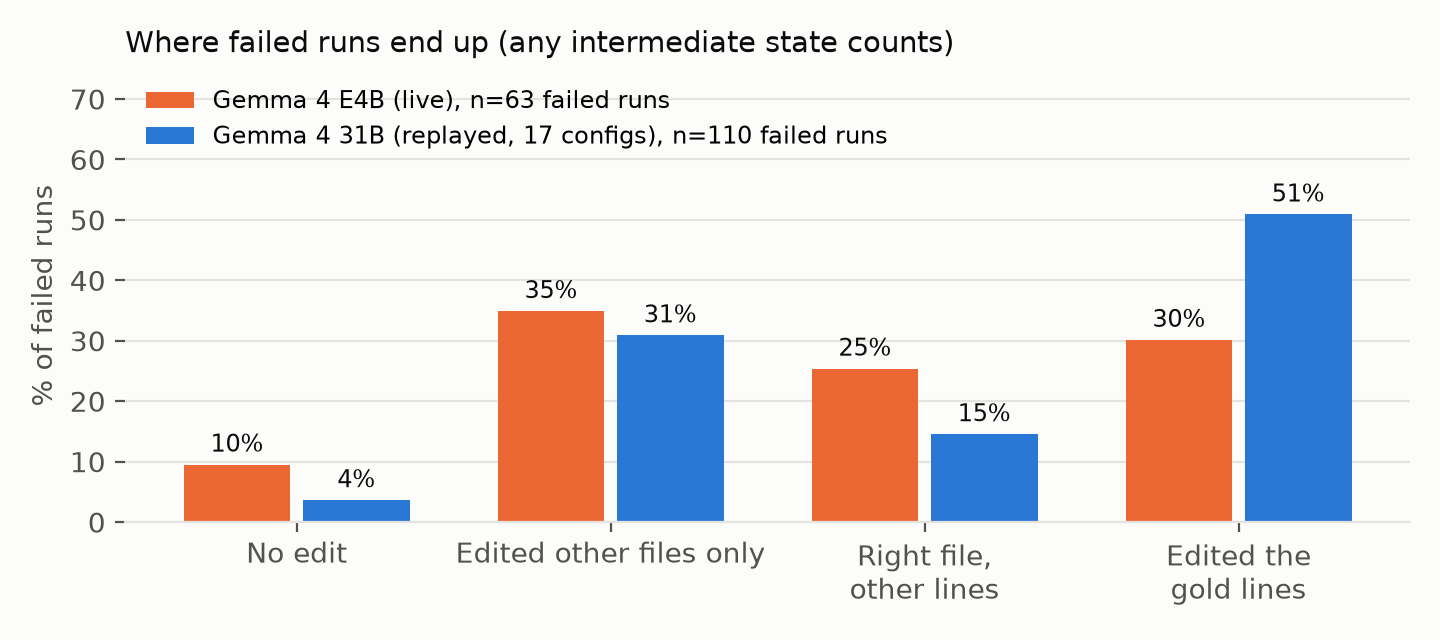
\includegraphics[width=\linewidth]{fig/fig1_reach.png}\caption{Where failed runs end up.}\end{figure}
Half of the failed 31B runs (56 of 110) edited the right lines at some point and still never produced a working version, close to the 60--69\% Kim et al. [1] report for frontier models. For E4B the share is 30\% (19 of 63). E4B's failures more often never touch the right file (44\%), so finding the right code is still its main problem.

\section*{What this means for building small agents}
\begin{enumerate}\setlength\itemsep{2pt}\item \textbf{Make the agent confirm its fix with the repository's real tests.} Our measurements say a pass from the project's suite is right about twice as often as a pass from a scratch script. A prompt rule or a skill that runs the relevant \texttt{tests/} files before submitting is cheap to add. This is a measurement, not yet a controlled experiment, and testing it directly is the obvious next step.\item \textbf{Do not stop at the first green result.} Early stopping on the agent's own check cost 13 fixes and gained none.\item \textbf{Do not build checkpoint-and-undo machinery for Gemma 4 yet.} There is almost nothing for it to recover, and 31B already reverts its own breaks.\item \textbf{Spend effort on reaching a fix.} For E4B that means finding the right file; for 31B, writing a correct change at the right place.\end{enumerate}
\section*{A new resource: scored agent states}
Most agent datasets label only the final patch. We release 1,431 intermediate workspace states from 345 Gemma 4 runs, each with its diff, the tool call that produced it, the agent's check results at that moment, and a pass or fail label from the official hidden tests. These are process-level labels: they say, step by step, whether the agent's work was correct. That makes them usable for training or evaluating verifiers and step-level reward models for small coding agents, and for testing stopping and selection rules offline. We also release the observation hook, the log replayer and the verification notebooks, so the same labels can be produced for any agent in this harness. Following the hosts' guidance, only derived data is shared: no problem statements, hidden tests or competition files.

\section*{Limitations}
\begin{itemize}\setlength\itemsep{2pt}\item The tasks come from two open-source libraries. The hidden competition set uses private repositories, and public-set results have been reported not to transfer [2].\item The 31B runs come from another team's 17 configurations, not the sample agent, so the size comparison also differs in agent setup and budget.\item "Working" inherits the tests' blind spots: 14.7\% of deliberately broken fixes still pass them [2].\item The check comparison is observational. Repository-suite checks may happen later in a run.\item We drop 25 of 298 logged runs whose final diff we could not rebuild exactly.\end{itemize}
\section*{Reproducibility}
Code, data and figures: \url{https://github.com/sundarshahi/gemma4-agents-rarely-lose-a-fix} (Apache-2.0). Each stage is a Kaggle notebook on the official harness: the live run with the observation hook, the log replay, the task audit, and the scoring. Three commands regenerate every number in this paper: \texttt{python analysis/analyze.py results/}, \texttt{python analysis/checks.py results/} and \texttt{python analysis/reach.py results/ results/gold\_hunks.json}. The analysis scripts include self-tests.

\textbf{Use of AI tools.} An AI assistant (Claude) helped write code and draft text. All numbers come from the released scripts, and the author checked the analysis and the final text.

\section*{References}\small
\noindent [1] M. Kim, D. Wang, S. Cui, F. Farmahinifarahani, T. Y. Zhuo, S. Garg, B. Ray, R. Mukherjee, V. Kumar. \emph{Coherence Collapse: Diagnosing Why Code Agents Fail After Reaching the Right Code.} arXiv:2603.24631, 2026.\par\smallskip
\noindent [2] M. Papasani. \emph{gemma4-agentic-swe: audit, ablations and traces for Gemma 4 agents.} github.com/TechNaom/gemma4-agentic-swe, commit 0758ce1, 2026. Apache-2.0.\par\smallskip
\noindent [3] C. E. Jimenez, J. Yang, A. Wettig, S. Yao, K. Pei, O. Press, K. Narasimhan. \emph{SWE-bench: Can Language Models Resolve Real-World GitHub Issues?} ICLR 2024. arXiv:2310.06770.\par\smallskip
\noindent [4] Gupta, Chaturvedi, Sengupta, Huan, Deoras. \emph{Dissecting model behavior through agent trajectories.} arXiv:2606.17454, 2026.\par\smallskip
\noindent [5] A. Cuadron et al. \emph{The Danger of Overthinking: Examining the Reasoning-Action Dilemma in Agentic Tasks.} arXiv:2502.08235, 2025.\par\smallskip
\noindent [6] A. Antoniades, A. Örwall, K. Zhang, Y. Xie, A. Goyal, W. Wang. \emph{SWE-Search: Enhancing Software Agents with Monte Carlo Tree Search and Iterative Refinement.} ICLR 2025. arXiv:2410.20285.\par\smallskip
\noindent [7] C. S. Xia, Y. Deng, S. Dunn, L. Zhang. \emph{Agentless: Demystifying LLM-based Software Engineering Agents.} arXiv:2407.01489, 2024.\par\smallskip
\noindent [8] R. Ehrlich, B. Brown, J. Juravsky, R. Clark, C. Ré, A. Mirhoseini. \emph{CodeMonkeys: Scaling Test-Time Compute for Software Engineering.} arXiv:2501.14723, 2025.\par\smallskip
\noindent [9] Vein05. \emph{Gemma 4 Gives Its Failing Patches Full Marks} (paper-track entry and code). github.com/Vein05/gemma4-paper-track, 2026.\par\smallskip
\noindent [10] pedronog8. \emph{Pre-registration: edit-state loss at context compaction.} Kaggle discussion 756850, 2026.\par\smallskip
\noindent [11] sigongjoa. \emph{Finds the File, Cannot Change It: Why a 2B Coding Agent Fails.} github.com/sigongjoa/gemma4-e2b-edit-failure, 2026.\par\smallskip
\end{document}
